\subsection{Placing an EAP file under version control}

If you already have an EAP file and would like to place it under version control, you first have to check it in as usual on the server using your favourite SVN
client. Once the project is checked in, the required .svn folder should be in the folder containing the EAP file. The next step is to register an SVN-variable
in EA:

\begin{enumerate}
  \item[$\blacktriangleright$] Open the EAP file, right click on a root folder and select ``Package Control'' and then ``Version Control Settings...''
  (Fig.~\ref{fig:advanced-topics-eaSVN-rightclick}).
  
\begin{figure}[!htbp]
\begin{center}
 	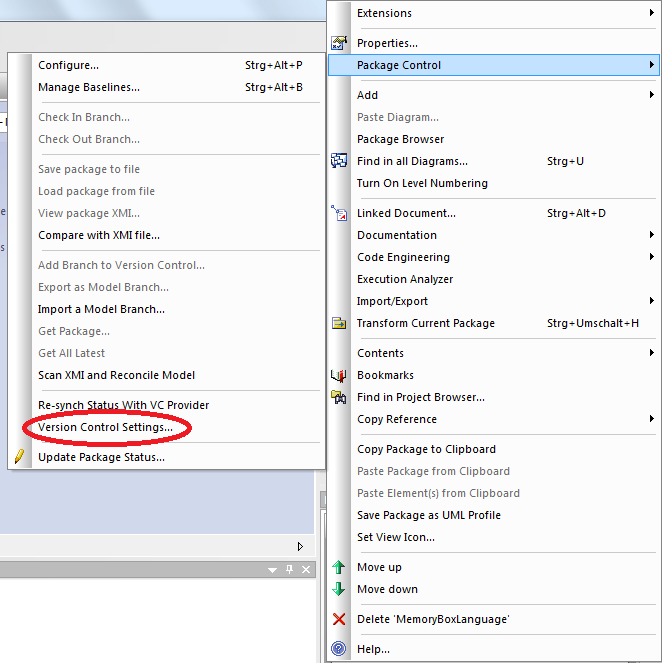
\includegraphics[width=0.7\textwidth]{rightclick}
	\caption{Select version control settings}
  	\label{fig:advanced-topics-eaSVN-rightclick}
\end{center}
\end{figure}

\newpage

  \item[$\blacktriangleright$] In the dialogue, choose a unique ID of your choice (we suggest you use the name of the EAP file) for the settings and activate
  the ``Subversion'' radio button below.
  
  \item[$\blacktriangleright$] Choose the local path to the folder which contains the EAP file in the ``Working Copy Path'' text-box.
  
  \item[$\blacktriangleright$] The field ``Workstation Settings'' must point to where you installed Sliksvn, i.e., \texttt{<path to
  SlikSVN>$\backslash$bin$\backslash$svn.exe")}. Press ``Save'' and close the dialogue (Fig.~\ref{fig:advanced-topics-eaSVN-variable}). If the dialogue closes
  without an error message, then you can be sure to have configured everything correctly.

\begin{figure}[!htbp]
\begin{center}
	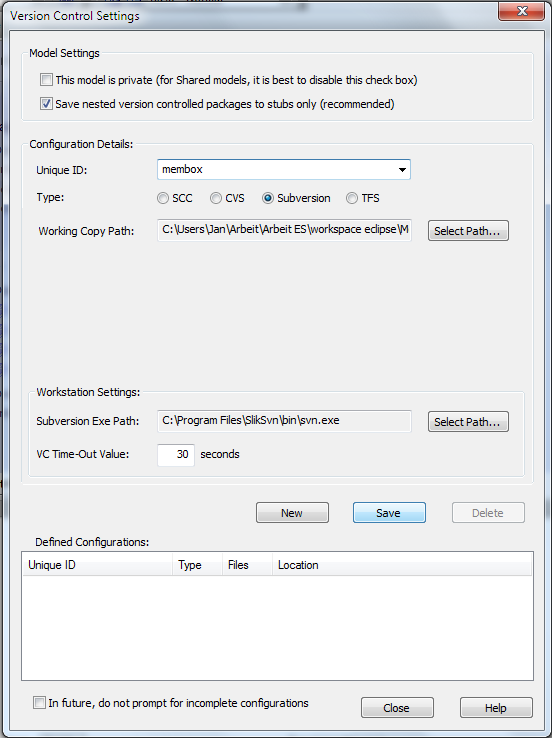
\includegraphics[width=0.8\textwidth]{versioncontrol}
	\caption{Register an SVN variable in EA}
  	\label{fig:advanced-topics-eaSVN-variable}
\end{center}
\end{figure}

\item[$\blacktriangleright$] In the EAP file, choose ``Package Control$\backslash$Configure...'' for \emph{each package} you wish to place under version control.

\newpage

\item[$\blacktriangleright$] In the ensuing dialogue, activate ``Control Package'' and select your previously defined SVN variable from the drop-down menu.
Enter the path where the XML file for the project should be placed. Although this is not enforced in any way, we recommend you create a folder structure that
mirrors the package structure in EA (Fig.~\ref{fig:advanced-topics-eaSVN-addPackage}). This process has to be repeated \emph{for all sub-packages} as soon as
their super-package has been placed under version control.

\vspace{0.5cm}

\begin{figure}[!htbp]
\begin{center}
	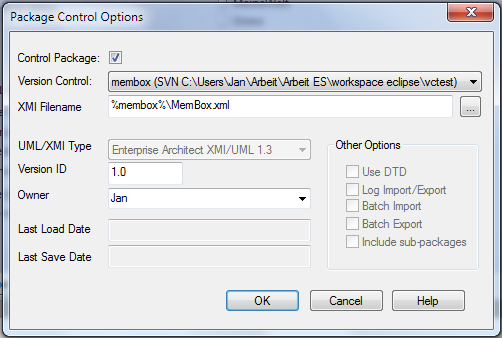
\includegraphics[width=0.8\textwidth]{cont}
	\caption{Placing a package under version control}
  	\label{fig:advanced-topics-eaSVN-addPackage}
\end{center}
\end{figure}

\item[$\blacktriangleright$] As a final step, check-in the current state of the EAP file directly with your SVN client.
As from this point, the EAP file should not be checked-in anymore, and all versioning actions should be performed via EA (and not directly with your SVN
client).

\end{enumerate}
